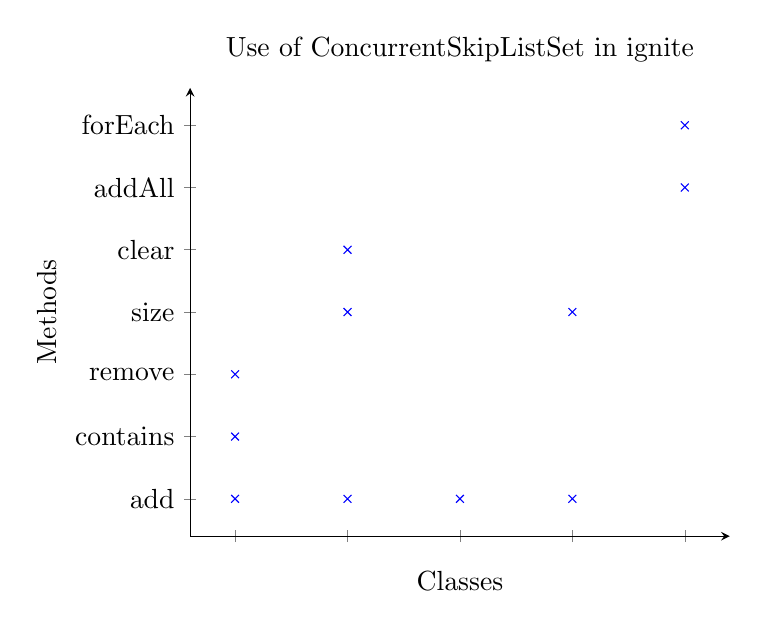
\begin{tikzpicture}
\begin{axis}[scatter/classes={U={mark=+,red}, NU={mark=x,blue}}, legend pos=outer north east,axis x line=bottom, axis y line=left, enlarge x limits=true, xlabel = {Classes}, ylabel = {Methods}, enlarge y limits=true, xtick = data, xticklabels = {,,},ytick=data, yticklabels={add,contains,remove,size,clear,addAll,forEach}, title={Use of ConcurrentSkipListSet in ignite}]
\addplot[scatter,only marks, scatter src=explicit symbolic]
coordinates {
(0,0) [NU]
(0,1) [NU]
(0,2) [NU]
(1,0) [NU]
(1,3) [NU]
(1,4) [NU]
(2,0) [NU]
(3,0) [NU]
(3,3) [NU]
(4,5) [NU]
(4,6) [NU]
};
\end{axis}
\end{tikzpicture}